\section{Problem and Approach}
\label{sec:description}

Here we will give a specification of the problem, and a detailed approach (i.e. the design of solution).
In order to simplify the problem and keep MLPs as simple as possible, one MLP will be used to check only the graphs (models) with a certain number of nodes and certain types of edges.
In other words, each type of graph will have its own MLP.
Notice that all the MLPs will have the same overall architecture.
The only difference will be the number of nodes at each layer.
That is only the bisimulation between graphs with the same scale will be studied.
The problem of the project become that if an MLP is possible to compute the bisimulation equivalence of two same scale models and how well it can do.
The basic steps of approach are as follows.
\begin{itemize}
    \item Generate a standard distinguishing algorithm.
    \item Based on the standard algorithm, develop a dataset generator.
    \item Construct MLPs that can accept graphs pairs and output judgement.
    \item Do experiments on the performance of the MLP with different training sets. \footnote{N.B. this step will be stated independently in Section \ref{sec:experiment}}
\end{itemize}


\subsection{Standard Bisimulation Algorithm}
For the first step, we will directly use the algorithm that solves the \emph{relational coarsest partition problem} \cite{Paige1987}, i.e. given the relation $E$ and initial partition $P$ over a set $U$ find the partition $P$ that \textquotedblleft every other stable partition is a refinement of it \textquotedblright.
From the perspective of set-theory, it is the same as solving bisimulation equivalence \cite{Dovier2004}.
Namely, if each block of the relational coarsest partition of the union of two graphs has nodes from both multi-directed graphs, these two graphs are bisimilar (see the set-perspective definition in Section \ref{sec:background}).
Moreover, compared with the algorithm given by Kanellakis and Smolka \cite{Milner1980}, their algorithm is more efficient in time (see Section \ref{sec:bac:bis}).
Yet, the algorithm given by Paige and Tarjan is not designed for multi-directed graphs.
It only processes the directed graph with only one kind of edges.
So by replacing every operation on one relation by a group of operations on each relation (see Step \ref{each_relation} in Algorithm \ref{alg:sbs}), the algorithm can be used for multi-directed graphs.
Here we give the description of the algorithm based on \cite{Paige1987}.

\begin{algor}\label{alg:sbs}
Standard Bisimulation Algorithm
\begin{enumerate}
    \item Get the union of two given graphs $U$.
    \item Initialise the partition $X$ and block set $C$, where $X=C=\{U\}$.
    \item Get the initial partition $Q$, by refine the only block $U$ in $Q$ with respect to $U$ itself. In other words, split $U$ on the preimage of itself, i.e. $Q = \{E^{-1}(U), U-E^{-1}(U)\}$, where $E$ is the any type of binary relation of nodes (also edges).
    \item Loop until block set $C$ is empty.
    \begin{enumerate}
        \item \label{loop} Pop the first block $s$ from block set $C$
        \item Check first two blocks of partition $Q$, that is contained in block $s$, make block $b$ be the smaller one.
        \item In partition $X$ split the block $s$ into block $b$ and block $s'=s-b$. if $s'$ is compound with respect to partition $Q$, add it back to block set $C$
        \item \label{each_relation} For each type of relation $E_i$, i.e. $i=1, i=2$ if there are two types of edges.
        Refine every blocks in partition $Q$ with respect to block $b$ and block $s'$.
        \item Add all blocks $x\in X$ that are compound with respect to partition $Q$ to block set $C$
    \end{enumerate}
    \item If there are nodes of both graphs in each block of partition $Q$ return true, else return false.
\end{enumerate}

\end{algor}

% \begin{defin}
% Concepts used in the algorithm. \footnote{All the definition here directly from \cite{Paige1987}}

% \begin{itemize}
%     \item $U$ is the union of two given graphs.
%     \item $S$ is the subset of $U$, i.e. $S \subseteq U$
%     \item $E$ is the links of $U$, which means edge $\langle x, y \rangle \in E $ (also denoted $xEy$).
%     \item For any subset $S$, $E(S) = \{y|\exists x \in S \text{ such that } xEy\}$ and $E^{-1}(S)=\{x|\exists y\in S \text{ such that } xEy \}$
%     \item If $B \subseteq U$, $B$ is \emph{stable} with respect to $S$ if either $S\subseteq E^{-1}(S)$ or $B\cap E^{-1}(S)=\emptyset$
%     \item If $P$ is a partition of $U$, $P$ is \emph{stable} with the respect to $S$ if all of the blocks belonging to $P$ are stable with respect to $S$.
%     \item $P$ is \emph{stable} if it is stable with respect to each of its own block.
% \end{itemize}
% \end{defin}
% This algorithm keep refine the a partition $Q$ (with the initial state that only contain $U$) until it is \emph{stable}.


\subsection{Test Case Generator}\label{sec:generator ds}
All the data used in this project is self-generated random and abstract without any human participation.
Here the model (multi-directed graph) generated will be represented as an expend adjacency matrix (see Figure \ref{fig:exp:model_represent}), where 1 stands for existence.
\begin{figure}[h]
    \centering
    \subfigure[Model]{
        \label{fig:example1_model}
        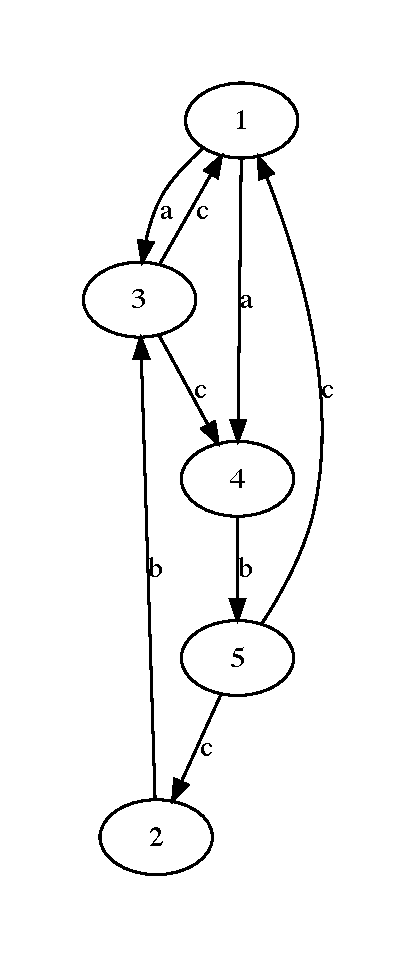
\includegraphics[width=2.0cm]{img/graph_example.pdf}}
    \subfigure[Adjacency Matrix]{
        \label{fig:example1_matrix}
        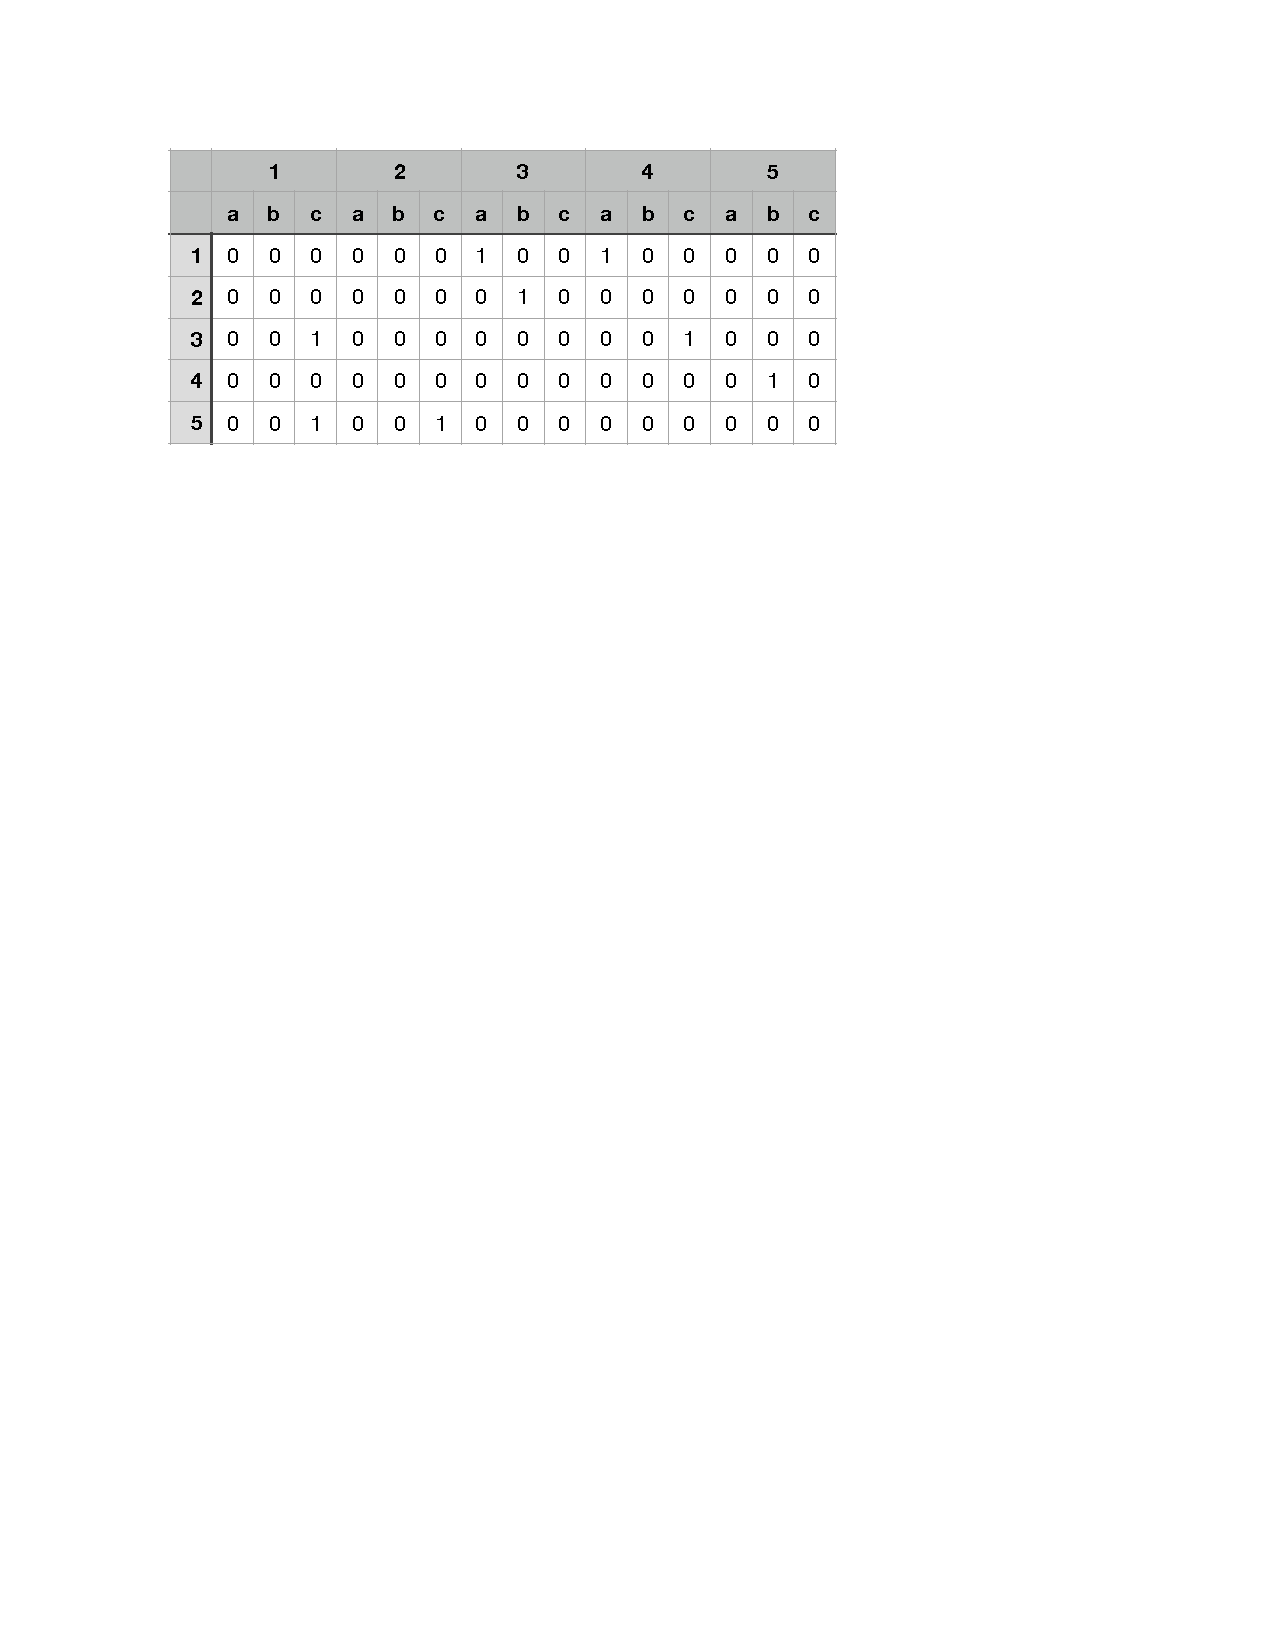
\includegraphics[width=0.6\textwidth]{img/example1_matrix.pdf}}
    \caption{Example model represent}
    \label{fig:exp:model_represent}
\end{figure}

There are two generators implemented.
However, only one is used in the final experiments (to be explained in Section \ref{sec:relisation})
The first idea is to randomly generate graphs.
Depends on the rate given, generate a bisimilar graph of another random non-bisimilar graph.
Then record them into the appointed file with flags.
Description of this algorithm is given as follow.
\begin{algor}
\label{alg:R_tcg}
Random Test Case Generator
\begin{enumerate}
    \item \label{item:gen_ran}Generate a random graph with certain scale, using the given density times a random number ($< 1$, $> 0$) as a probability of each possible edge.
    \item According given rate of positive cases and negative cases, decide to generate a bisimilar graph (jump to Step \ref{item:bi}) or non-bisimilar graph (jump to Step \ref{item:non_bi}).
    \item \label{item:non_bi} Keep generate random graph like Step \ref{item:gen_ran} and check the bisimulation equivence, until they are not (then jump to Step \ref{item:convert}).
    
    \item \label{item:bi}Get the \emph{relational coarsest partition} $P_\text{origin}$ of given graph.
    \item Randomly divides the nodes of the new graph into the same partition $P_\text{similar}$, i.e. the partition that has the same number of blocks (N.B. the length of each block not necessary to be same).
    \item Assemble the minimum bisimilar graph, where each block of its partition contains only one node. 
    \item \label{item:bi_end}For each edge of the minimum graph, generate a random number ($\geq 1$) of edges between the random nodes from two corresponding blocks of $P_\text{similar}$ respectively.
    
    \item \label{item:convert}Convert the new generated graph into adjacency matrix.
    \item Write two graphs with flag into file (jump to Step \ref{item:gen_ran} if there are not enough test cases).
\end{enumerate}
\end{algor}

However, the test cases generated may not actually random, which may have some superficial features that are easy to be caught by the later MLP (to be described in Section \ref{sec:des:ml}).
For example the heuristic algorithm for generate bisimilar graph (see Algorithm \ref{alg:R_tcg}, Step \ref{item:bi} to Step \ref{item:bi_end}) may have some kind of inclination.
To get rid of these potential bias, a full case generator is designed.
This generator can generate all possible graphs in given scale and record all possible combinations with flags.
The basic idea of iteration is that since a graph can be seen as an adjacency matrix, it can be represented as a binary string.
By counting in binary, all possible graphs on the same scale can be traversed.
Here gives the description of this algorithm.
\begin{algor}
\label{alg:F_tcg}
Full Test Case Generator
\begin{enumerate}
    \item For every graph, calculate its minimum bisimilar graph. Meanwhile, construct a dictionary where the key is the minimum bisimilar graph and the value is a set of all graphs that are bisimilar, i.e. have the same minimum bisimilar graph which is their key.
    \item According to the dictionary, catalogue all the graph (graphs with the same key will have the same label).
    \item Go through all graphs again, generate all combinations with flag base on their label.
\end{enumerate}
\end{algor}

\subsection{MLP Structure}
\label{sec:des:ml}
After the test case generator produces data, the network should be trained.
The structure is designed to be as simple as possible.
Combine with the process step of the standard algorithm, the network is structured to meet the process (see Figure \ref{fig:mlp_model}).
The first layer is the input layer, which will accept fixed length binary (i.e. adjacency matrix).
In order to push the network to get the abstraction, the second layer called re-represent layer has fewer neurons than the input layer. 
And the first two layers are divided into two independent parts that share parameters (see Part 1 and Part 2 in Figure \ref{fig:mlp_model}).
Each part will accept one graph.
The distinguishing part will accept input from two graphs and get the conclusion about bisimulation equivalence, i.e. output the probability of positive and negative.
There are three reasons to design a network like that.
First is by sharing the parameters, the overall training will be master.
The second reason is that it solves the problem of sequence, i.e. the output will not be affected by the priority of two graphs.
The third reason is that this kind of modular design will be much easier for reuse, e.g. used as part of the graph simplify the network.

\begin{figure}[h]
    \centering
    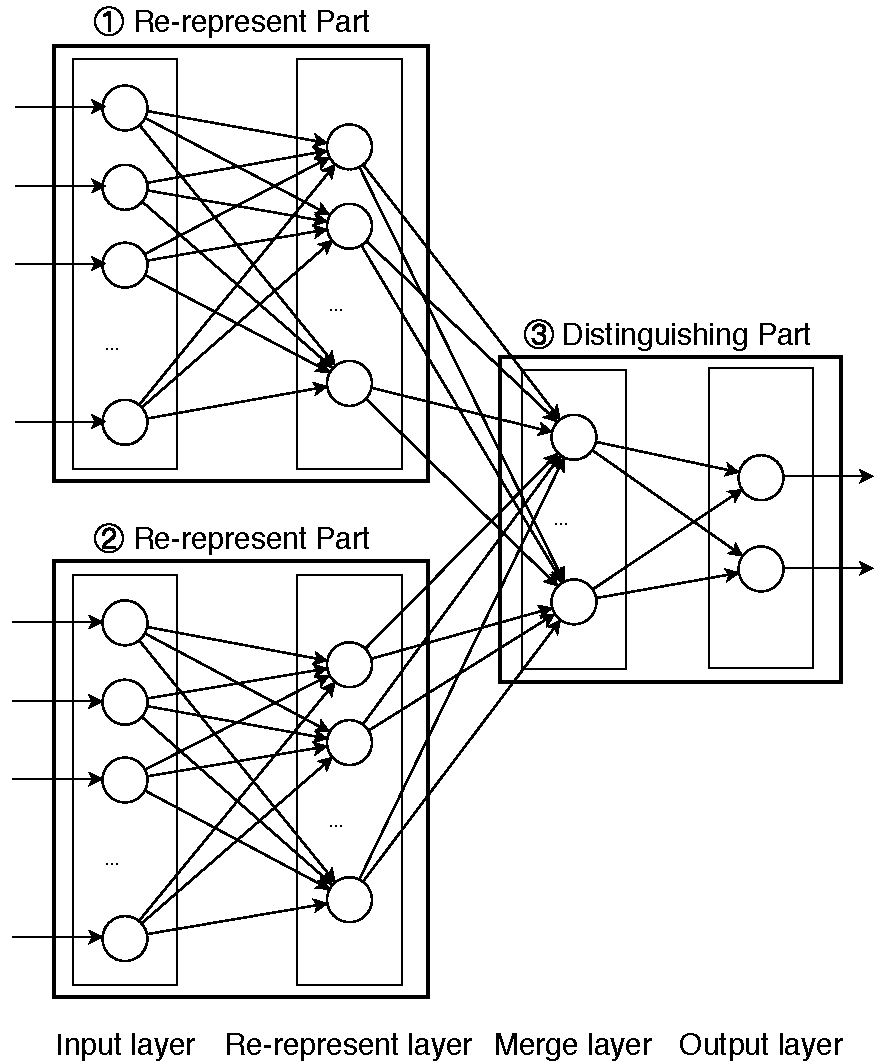
\includegraphics[width=0.65\textwidth]{img/mlp.pdf}
    \caption{MLP model}
    \label{fig:mlp_model}
\end{figure}

\subsection{General Structure}
The design of the general structure is aimed at developing a reusable tool.
Thus the structure is very simple and highly modularised (see Figure \ref{fig:general_str}).
Dataset generator and ML-algorithm is packed independently.
And each module can be called in a python program or used as a command line tool directly by the user.
\begin{figure}[h]
    \centering
    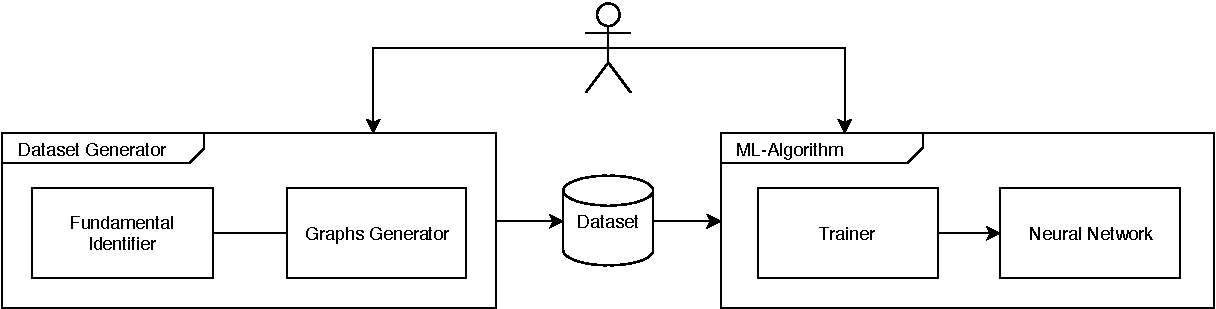
\includegraphics[width=\textwidth]{img/architecture.pdf}
    \caption{General structure}
    \label{fig:general_str}
\end{figure}

